\documentclass[xcolor=dvipsnames, aspectratio = 169]{beamer}
\usepackage[english]{babel} %% english
\usepackage[utf8]{inputenc}
\usepackage[T1]{fontenc}
\usepackage{include/chariteBeamer}
\usepackage{hyperref}
\usepackage{blkarray}
\author[E. Sprünken]{Erin Sprünken}
\institute[]{
Institut für Biometrie und Klinische Epidemiologie\\[1Ex] 
Charité - Universitätsmedizin Berlin, Berlin\\[1Ex]
erin-dirk.spruenken@charite.de} 
\titlegraphic{\pgfuseimage{frontUnilogo}}

\tikzset{>=latex}
%\usepackage{amsmath}
%\usetikzlibrary{shadows}
\usepackage[edges]{forest}
\usetikzlibrary{positioning}
\usepackage{biostat}
\setbeamertemplate{caption}[numbered]
\let\qed\relax
\forestset{declare toks={elo}{}}
%% ================================================================== %% 

\author[L. Mödl, M. Becher, E. Sprünken]{Lukas Mödl, Matthias Becher, Erin Sprünken} 
\title{R-Kurs: Tag 4} 
\date[]{\today}

%% ================================================================== %% 
\setbeamercolor*{mycol}{bg=chariteGray, fg=chariteBlue}

\hyphenation{Sam-ples}
\begin{document}

%% ================================================================== %%
%% ================================================================== %%
\setbeamertemplate{footline}{\begin{tikzpicture}
    \node [inner sep=0pt, anchor=east] (0,0) {
      
\includegraphics[width=\paperwidth,height=0.7cm]{include/charite_footer}};
    \node [inner sep=0pt, anchor=east] at (-0.5ex,-0ex){};
\end{tikzpicture}}

\setbeamertemplate{headline}{
%\leavevmode
\hspace{-0.49em}\hbox{
	\begin{beamercolorbox}[wd=1.02\paperwidth,ht=2.25ex,dp=1ex,left]{mycol}%
    \usebeamerfont{section in head/foot}
  \end{beamercolorbox}%
}}
{
  \usebackgroundtemplate{ \hspace{-0.5em}\begin{tikzpicture}
  \node[opacity=0.7, anchor=south] (0,0) {
\includegraphics[height=\paperheight, width=1.04\paperwidth]{include/frontmatter.pdf}};
  \end{tikzpicture}
} 
%\frame{\titlepage}
\begin{frame}
\centering
	\vspace{4em}
	{\Large \textcolor{chariteBlue}{\inserttitle}}\\
	 \vspace{1em}
	{\Large \textcolor{black}{\insertauthor \\}} 
	\vspace{2em}
	{\footnotesize \textcolor{black}{\insertinstitute \\\vspace{1em} \insertdate}} 
	\vspace{0em}
	\begin{figure}[h!]
		
\includegraphics[width=5cm]{include/Charite_Logo.png}
	\end{figure}
%	\pgfuseimage{frontUnilogo}
\end{frame}
}
%% ================================================================== %%

\setbeamertemplate{footline}{\begin{tikzpicture}
    \node [inner sep=0pt, anchor=east] (0,0) {
      
\includegraphics[width=\paperwidth,height=0.7cm]{include/charite_footer}};
    \node [inner sep=0pt, anchor=east] at (-0.5ex,-0ex) {\tiny \insertframenumber{}$\,$|$\,$\inserttotalframenumber};
\end{tikzpicture}}

\setbeamertemplate{headline}{%
%\leavevmode%
\hspace{-0.49em}\hbox{
	\begin{beamercolorbox}[wd=.68\paperwidth,ht=2.25ex,dp=1ex,left]{mycol}%
    \usebeamerfont{section in head/foot}\hspace*{1em}
  \end{beamercolorbox}%
  \begin{beamercolorbox}[wd=.20\paperwidth,ht=2.25ex,dp=1ex,right]{mycol}%
    \usebeamerfont{author in head/foot}\insertshortauthor
  \end{beamercolorbox}%
  \begin{beamercolorbox}[wd=.14\paperwidth,ht=2.25ex,dp=1ex,center]{mycol}%
    \usebeamerfont{date in head/foot}\insertdate
  \end{beamercolorbox}%
  }
}


\frame{\tableofcontents}

\setbeamertemplate{headline}{%
%\leavevmode%
\hspace{-0.49em}\hbox{
	\begin{beamercolorbox}[wd=.68\paperwidth,ht=2.25ex,dp=1ex,left]{mycol}%
    \usebeamerfont{section in head/foot}\hspace*{1em}\thesection. \  \insertsectionhead
  \end{beamercolorbox}%
  \begin{beamercolorbox}[wd=.20\paperwidth,ht=2.25ex,dp=1ex,right]{mycol}%
    \usebeamerfont{author in head/foot}\insertshortauthor
  \end{beamercolorbox}%
  \begin{beamercolorbox}[wd=.14\paperwidth,ht=2.25ex,dp=1ex,center]{mycol}%
    \usebeamerfont{date in head/foot}\insertdate
  \end{beamercolorbox}%
  }
}



\section{\textsf R Pakete}


\begin{frame}[fragile]{Installation weiterer \textsf R Pakete}
    Jede \textsf R Umgebung installiert und lädt standardmäßig die Pakete \texttt{base}, \texttt{stats}, \texttt{datasets}, \texttt{methods} und \texttt{graphics}.\bigskip
    \begin{itemize}
        \item Installation weiterer Pakete mit:
        \begin{verbatim}
        install.packages("name-des-pakets", dependencies = TRUE)
        \end{verbatim}
        \item Bei jedem Start von \textsf R muss das Paket, wenn es verwendet werden soll, geladen werden:
        \begin{verbatim}
        library("name-des-pakets")
        \end{verbatim}
        \item Aktualisieren der Pakete mit:
        \begin{verbatim}
        update.packages()
        \end{verbatim}
    \end{itemize}
\end{frame}

\begin{frame}{Beispiel: Installation und Laden des \textsf R Pakets \texttt{MASS}}
    \begin{center}
        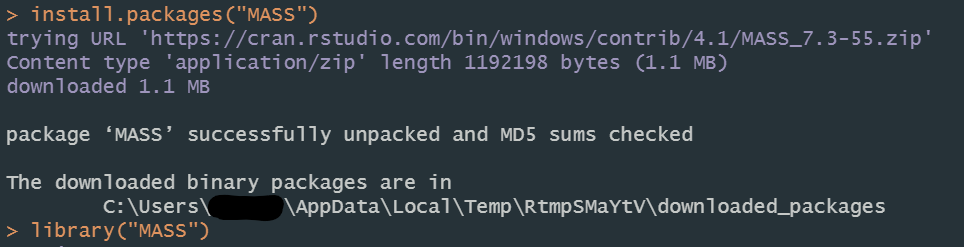
\includegraphics[width=\textwidth, keepaspectratio]{pakete.png}
    \end{center}
\end{frame}

\begin{frame}[fragile]{Empfehlenswerte Pakete}
      \begin{itemize}
          \item \verb+MatchIt+ für Propensity Score Matching 
          \item \verb+MASS+ für Negativ-binomiale Regression \\
          \item \verb+lmer+ bzw. \verb+lme4+ für Mixed-Models \\
          \item \verb+pwr+ für Power-Analyse und insbesondere zur Fallzahlplanung \\
         \item \verb+ggplot2+ für schöne Plots \\
      \item \verb+foreign+ für das Einlesen von \verb+.sav+-Dateien \\ 
      \item ...
   \end{itemize}
\end{frame}

\section{Programmierung I: if-else-Anweisung}

\begin{frame}[fragile]{Konzeption if-Anweisung}
    Möchte man einen Codeblock abhängig von einem bestimmten Wert ausführen oder nicht, muss eine if-Anweisung verwendet werden. if-Anweisungen definieren einen Codeblock, der nur dann ausgeführt wird, wenn die übergebene Bedingung wahr ist.\bigskip\\
    
\begin{tikzpicture}[node distance=8cm, auto]
      \node[rectangle, draw] (condition) {Bedingung};
      \node[rectangle, draw, right of=condition] (res2) {Code im if-Block wird ausgeführt};
      \draw[draw, ->] (condition) -- node {ist erfüllt} (res2);
    \end{tikzpicture}
\end{frame}

\begin{frame}[fragile]{Beispiel: Bedingte Ausgabe}
  \begin{verbatim}
      x = 2
      
      if(x <= 3)
      {
          print("x ist kleiner als 3")
      }
  \end{verbatim}
\end{frame}

\begin{frame}[fragile]{Konzeption if-else-Anweisung}
    Bei der if-Anweisung wird der Code, der nach der if-Anweisung steht immer ausgeführt. Das ist in einer Entweder-Oder-Situation natürlich nicht wünschenswert. Hier schafft die if-else-Anweisung Abhilfe.\bigskip\\
    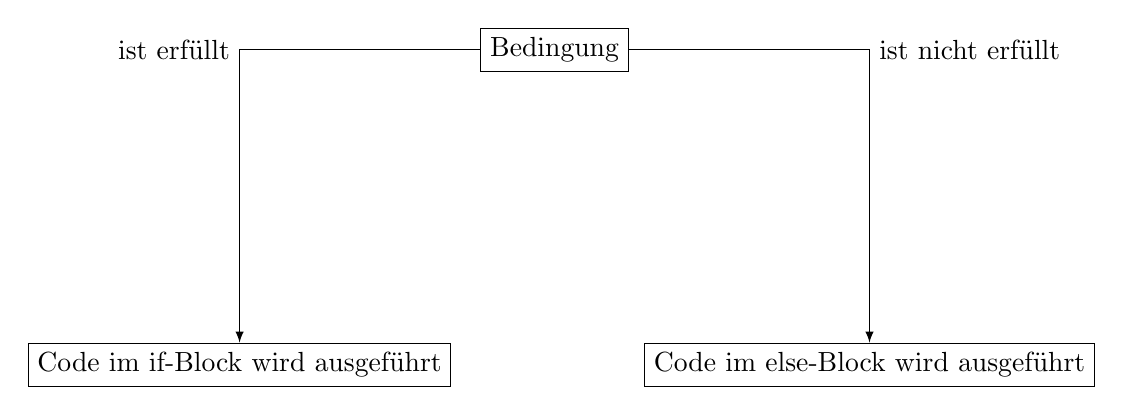
\begin{tikzpicture}[node distance=4cm, auto]
      \node[rectangle, draw] (condition) {Bedingung};
      \node[below of=condition] (state) {};
      \node[rectangle, draw, left of=state] (res1) {Code im if-Block wird ausgeführt};
      \node[rectangle, draw, right of=state] (res2) {Code im else-Block wird ausgeführt};
      \draw[draw,->] (condition) -| node[anchor=west] {ist nicht erfüllt} (res2);
      \draw[draw,->] (condition) -| node[anchor=east] {ist erfüllt} (res1);
    \end{tikzpicture}
\end{frame}

\begin{frame}[fragile]{Beispiel: Bedingte Ausgabe}
    \begin{verbatim}
      x = 2
      
      if(x <= 3)
      {
          print("x ist kleiner als 3")
      }
      else
      {
          print("x ist größer als 3")
      }
    \end{verbatim}
\end{frame}

\section{Programmierung II: Schleifen}

\begin{frame}[fragile]{Konzeption \texttt{for}-Schleife}
    Eine beiden wesentlichen Schleifen in \textsf R ist die \texttt{for}-Schleife. \texttt{for}-Schleifen führen einen Codeblock so oft aus, wie eine definierte Laufvariable Werte in einer Indexmenge annehmen kann. \bigskip\\
    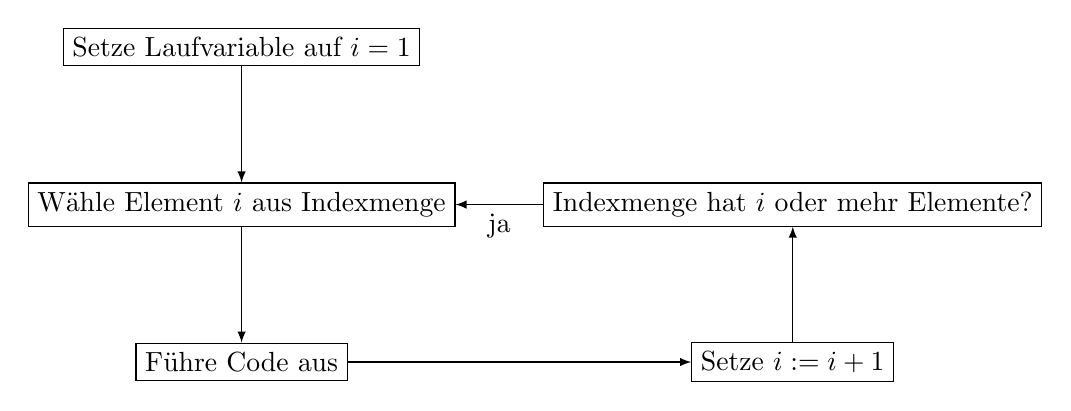
\begin{tikzpicture}
      \node[rectangle, draw] (init) {Setze Laufvariable auf $i=1$};
      \node[rectangle, draw, below of=init, node distance=2cm] (start) {Wähle Element $i$ aus Indexmenge};
      \node[rectangle, draw, below of=start, node distance=2cm] (code) {Führe Code aus};
      \node[rectangle, draw, right of=code, node distance=7cm] (index) {Setze $i:=i+1$};
      \node[rectangle, draw, right of=start, node distance=7cm] (check) {Indexmenge hat $i$ oder mehr Elemente?};
      \draw[draw,->] (init) -- (start);
      \draw[draw,->] (start) -- (code);
      \draw[draw,->] (code) -- (index);
      \draw[draw,->] (index) -- (check);
      \draw[draw,->] (check) -- node[anchor=north] {ja} (start);
    \end{tikzpicture}
\end{frame}

\begin{frame}[fragile]{Konzeption \texttt{while}-Schleife}
Die andere wesentliche Schleife ist die \texttt{while}-Schleife. Im Gegensatz zur \texttt{for}-Schleife wird hier ein Codeblock so lange ausgeführt, wie eine übergebene Bedingung wahr ist.\bigskip\\
    \begin{center}\begin{tikzpicture}
      \node[rectangle, draw, below of=init] (start) {Bedingung};
      \node[rectangle, draw, below of=start, node distance=4cm] (code) {Führe Code aus};
      \draw[draw,->] (start) -- node[anchor=east]{ist erfüllt} (code);
      
      \draw[draw, ->] (code) --++ (2cm,0cm) |- (start);
    \end{tikzpicture}\end{center}
\end{frame}

\begin{frame}[fragile]{Beispiel I: Einfacher \texttt{for}-Schleife}
    \begin{verbatim}
        indexmenge = seq(1, 10, by = 1)
        
        for(i in indexmenge) 
        {
        
            print(i)
            
        }
   \end{verbatim}
\end{frame}

\begin{frame}[fragile]{Beispiel II: Einfache \texttt{while}-Schleife}
    \begin{verbatim}
        a = 10
        b = 0
        
        while(a > b) 
        {
            a = a - 0.5
            b = b + 0.5
            
            print("a = ")
            print(a)
            print("b = ")
            print(b)
        }
    \end{verbatim}
\end{frame}

\begin{frame}[fragile]{Achtung vor unendlichen Schleifen!}
    \begin{verbatim}
        a = 10
        b = 0
        
        while(a > b) 
        {
            
            a = a + 1
            
        }
    \end{verbatim}
    Diese Schleife endet nie! Zum Abbruch muss ``ESC'' gedrückt werden.
\end{frame}

\begin{frame}[fragile]{Beispiel III: Berechnung des Standardfehlers mittels Monte-Carlo Simulation}
    \begin{verbatim}
        n <- 1000
        stichprobe <- rnorm(n, 5, 2)
        mittelwerte <- numeric(n)
        
        for(i in seq(1, n, by = 1)) 
        {
            s <- sample(stichprobe, size = n, replace = TRUE)
            mittelwerte[i] <- mean(s)
        }
        
        standardfehler <- sd(mittelwerte)
    \end{verbatim}
\end{frame}

\section{Eigene Funktionen}

\begin{frame}[fragile]{Konzeption eigener Funktionen}
    Bisher haben wir nur vordefinierte Funktionen wie beispielsweise \texttt{t.test} verwendet. \textsf R erlaubt es aber auch, eigene Funktionen zu schreiben.\bigskip
    \begin{verbatim}
        meine_funktion <- function(<argumente>) 
        {
            
            <code>
            
            return(<funktionswert>)
        } 
    \end{verbatim}
\end{frame}

\begin{frame}[fragile]{Beispiel I: Eine Funktion mit einem Argument}
    \begin{verbatim}
        f <- function(x)
        {
            y <- x^2
            
            return(y)
        }
    \end{verbatim}
\end{frame}

\begin{frame}[fragile]{Beispiel II: Eine weitere Funktion mit einem Argument}
    \begin{verbatim}
        wochentag <- function(x) 
        {
            
            return(format(as.Date(x, "%d.%m.%Y"), "%A"))
            
        }
    \end{verbatim}
\end{frame}

\begin{frame}[fragile]{Funktionen werden wenn möglich vektorisiert}
    \begin{verbatim}
        daten <- c("8.5.1949", "5.3.1995", "1.1.2000", "1.1.2022")
        
        > wochentag(daten)
        
        [1] "Mittwoch" "Mittwoch" "Samstag" "Samstag"
    \end{verbatim}
\end{frame}

\begin{frame}[fragile]{Beispiel III: Eine Funktion mit zwei Argumenten}
    \begin{verbatim}
        bmi_rechner <- function(gewicht, groesse) {
            
            # gewicht in kg
            # groesse in m
            
            bmi <- gewicht / groesse^2
            
            return(bmi)
        }
    \end{verbatim}
\end{frame}

\begin{frame}[fragile]{Default Werte für Argumente vergeben}
        \begin{verbatim}
        bmi_rechner <- function(gewicht, groesse = 1.82) 
        {
            # gewicht in kg
            # groesse in m
            
            bmi <- gewicht / groesse^2
            
            return(bmi)
        }
    \end{verbatim}
\end{frame}

\begin{frame}[fragile]{Funktion für den BMI Rechner verbessern}
        \begin{verbatim}
        bmi_rechner <- function(gewicht, groesse = 1.82) 
        {
            # gewicht in kg
            # groesse in m
            
            if(gewicht <= 0 | groesse <= 0)
            {
              stop("Gewicht und Größe dürfen nicht <= 0 sein!")
            }
            else
            {
              bmi <- gewicht / groesse^2
              return(bmi)
            }
    \end{verbatim}
\end{frame}

\end{document}
